\chapter{実装}
\label{chap:implementation}

\section{実装の概要}

本研究では,RDMAを用いて,動作中のマシンのメモリの値を取得していくことで,リモートホストから監視対象ホストのオペレーティングシステムのコンテキストを復元していくことを目指す.
この目的を実現するために,本研究では,nettlpを用いて実験を行う.

\section{nettlp}
\label{section:nettlp}

nettlp本来の目的は,PCIeデバイスの開発プラットフォームである.(リファレンス)

その機能の一つとして,DMA messageとethernetパケットを相互変換する機能がある.
\ref{chap:related_works}で述べたが,RDMAのInfiniband実装は,制限が多い.(もう少し詳しく)
nettlpにおけるRDMAでは,物理アドレスを指定することで,任意のバイト数(なんバイトだっけ?)の値を取得することが可能である.
また,アクセスできないメモリアドレスは存在しない,すなわち全メモリアドレス空間から値を取得することが可能となっている.

nettlpはFPGAボード上で動作するものであり,これを利用するためのインターフェースとして,libtlpが用意されている.
libtlpでは,RDMAを用いてメモリダンプを取得するためのインターフェースが関数として用意されている.
この関数を含んだヘッダファイルをincludeし,プログラムから呼び出すことで,メモリアドレスの値が返ってくる.

用意されている関数は,\verb|dma_read|関数と\verb|dma_write|関数の二つである.
\verb|dma_read|関数は,値を読みだすための関数であり,呼び出す際に読みたいメモリアドレスを渡す.
\verb|dma_write|関数は,値を指定した物理アドレスに書き込むための関数であり,呼び出す際に,書き込みたいメモリアドレスと値を渡す.

本研究では,\verb|dma_read|関数のみを用いる.

\subsection{process-list.c}

このファイルでやっていることをかく.

\section{実験環境}

本研究で実装を行う環境は,図\ref{fig:zentai}にあるように,nettlpが書き込まれたFPGAが刺さった監視対象ホストと,本研究における実装を実行するホストの2台で構成する.

監視対象ホストは,Linux 4.15.0-72-genericのubuntuであり,PCIeデバイスとして,nettlpが書き込まれたFPGAボードが刺さっている.
本研究では,FPGAボードとして,ザイリンクスのやつを使用している.
また,このFPGAボードは,ネットワークインターフェースでもあり,IPアドレスとして,192.168.10.1を静的に振ってある.

実装を実行するホストは,Linux 4.19.0-6-amd64のDebian busterであり,光ファイバーケーブル(名称はあとで修正)が刺さるNICを刺している.以後,実装ホストと呼称する.
このNICにはIPアドレスとして,192.168.10.3を静的に振ってある.
監視対象ホストに対してRDMAを実行する際は,\verb|dma_read|関数,あるいは\verb|dma_wirte|関数を通して192.168.10.1に対してIPパケットを送信している.

\begin{figure}[htbp]
    \caption{全体}
    \label{fig:zentai}
    \begin{center}
        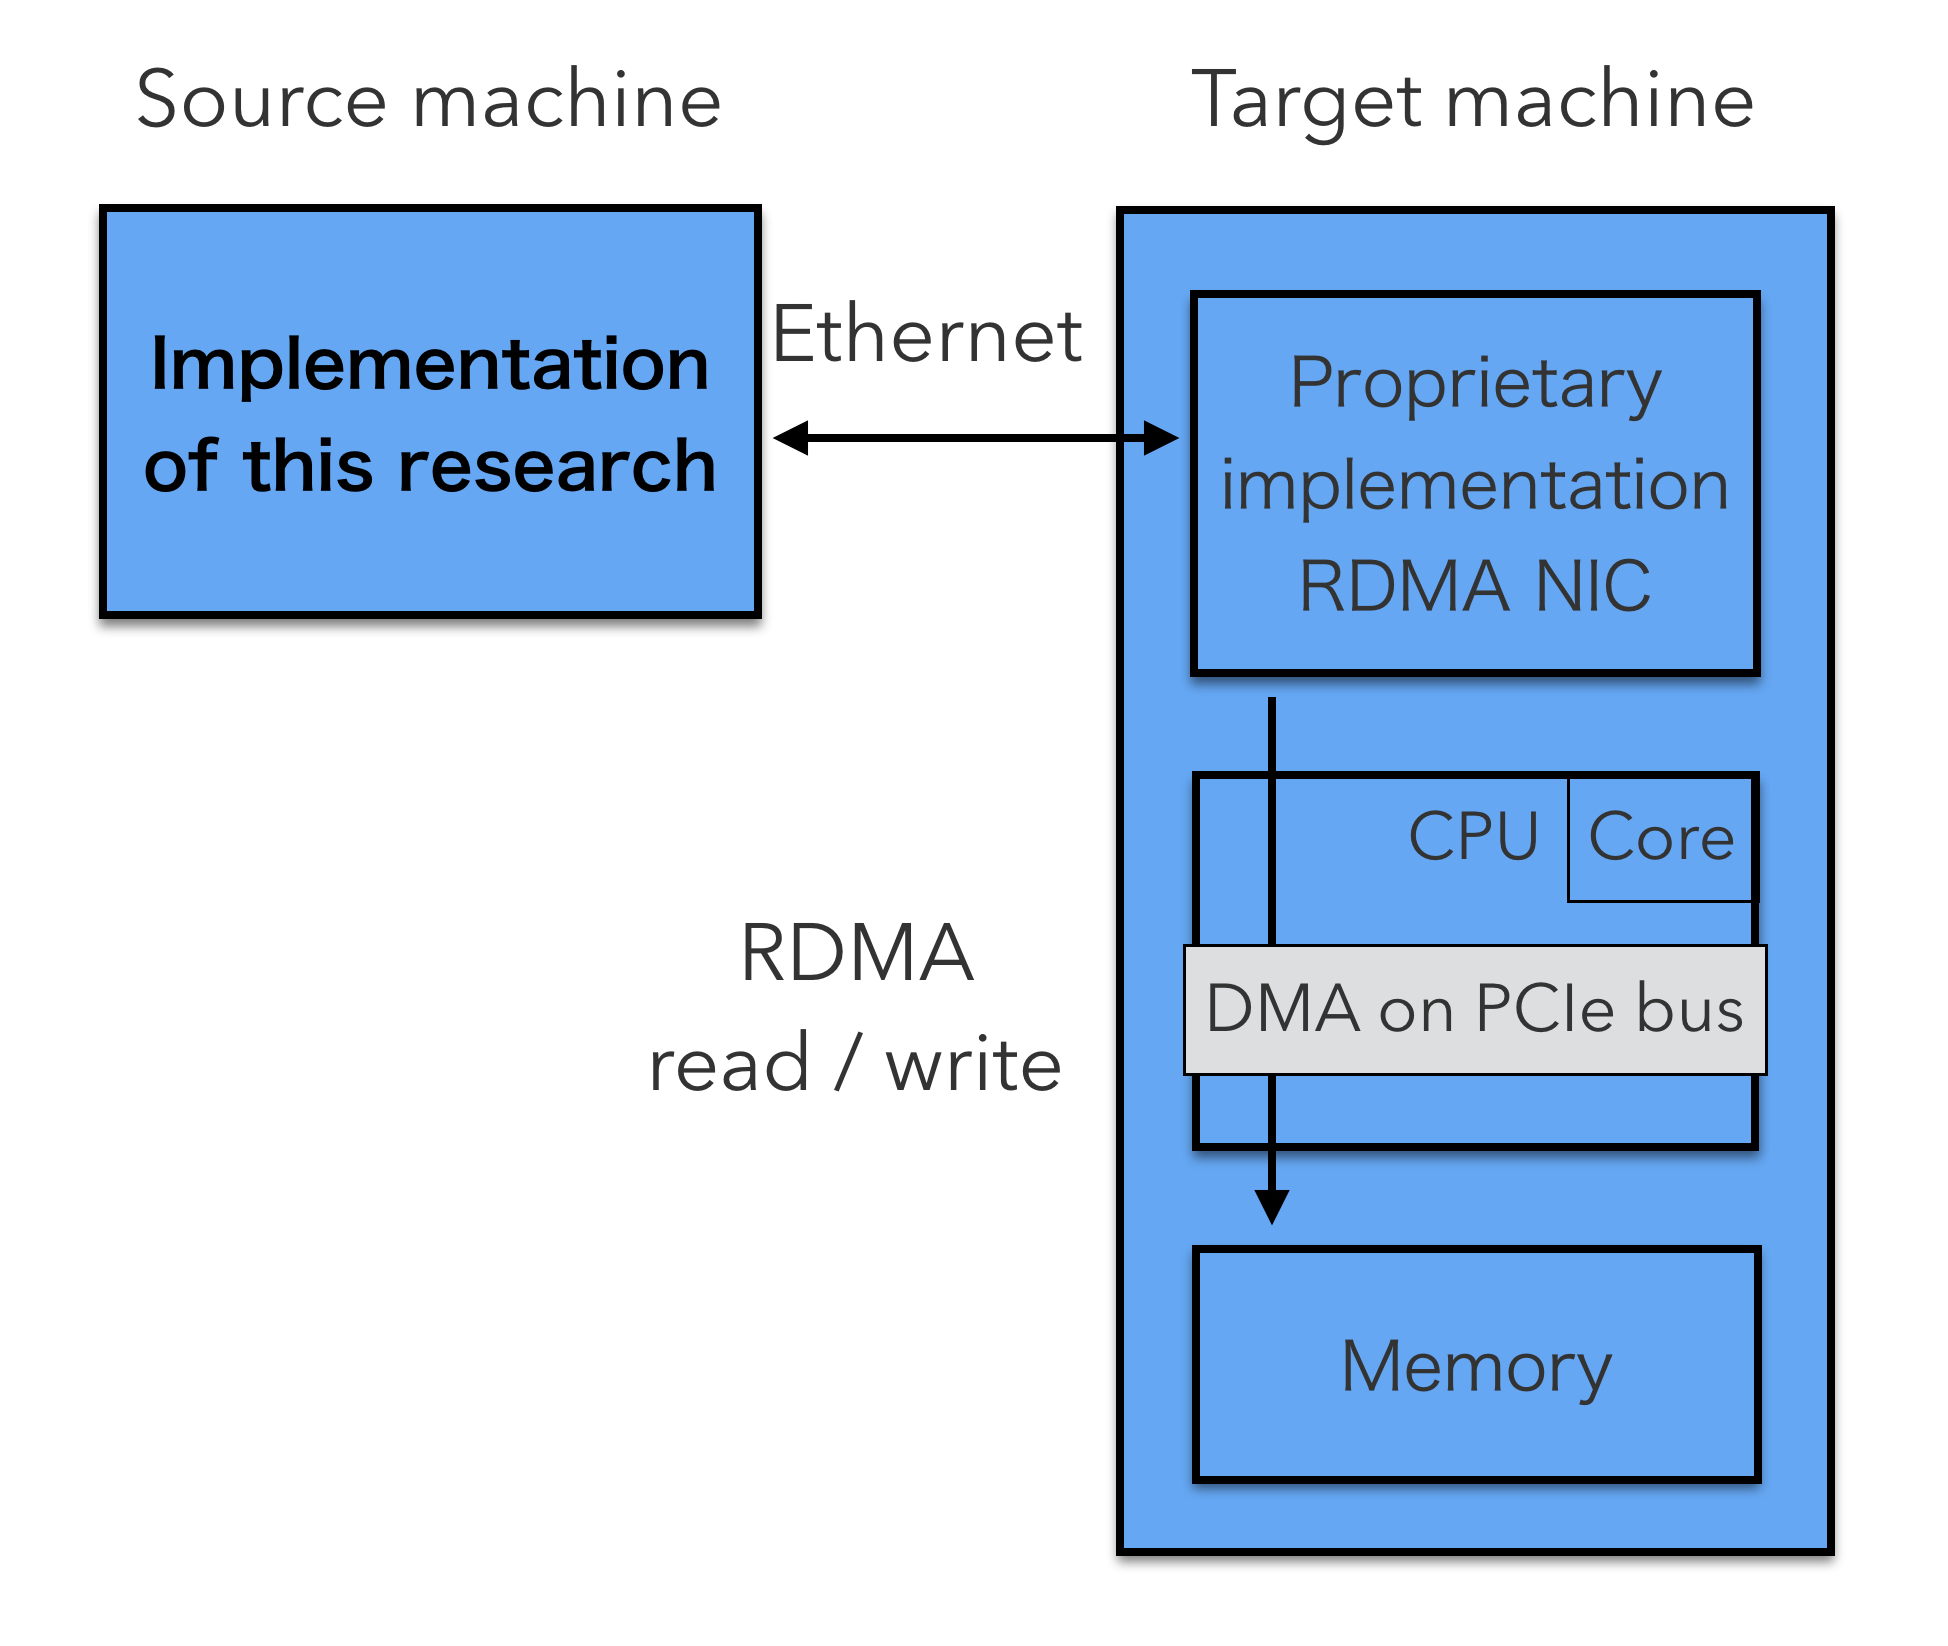
\includegraphics[bb=0 0 1000 800,width=15cm]{img/zentai.png}
    \end{center}
\end{figure}

\section{実装の前提情報}

本研究では,Linuxカーネルのバージョンは,実装ホストは知っている情報とする.
\label{section:want}で述べたもののうち,Linuxカーネルのバージョンだけは一旦Givenでやる.

\section{実装の全体}

ダンプしてくるということを書く.物理アドレスのマッピングに関しても

実験における第一段階として,\ref{section:want}で述べたように,監視対象ホストのカーネルコンフィグおよび\verb|init_task|の仮想アドレスを知ることを目指す.
そこで,本研究では,この情報をメモリ上から探す.\ref{section:mem_dump}で述べる実装では,取得できるメモリダンプを全て取得し,解析する手法に関して述べる.

次の工程として,それをリストアップ.

次の工程として,収集したカーネルコンフィグを元に手元のコンピュータでLinuxカーネルのソースコードに対してプリプロセスの処理を行い,\verb|task_struct|型を確定する.
さらに,ソースコード上にある\verb|__phys_addr|関数の実体を収集する.

最後に,この工程で得られた情報をもとに,libtlpで提唱されている手法を用いて,プロセスの一覧を正しく取得できることを確認する.

\subsection{mem\_dump}
\label{section:mem_dump}

第一の工程として,メモリの全ての情報を取得する.ソースコードは以下である.この実装を実装ホストで実行し,出力結果をファイルに格納する.
この実装では,libtlpを通して,監視対象ホストのメモリを全探索する.この実装の実行には長い時間(何分?)かかるため,アトミックな情報ではない.
そのため,ここで取得したメモリダンプは,解析には使えない.
ここで取得したメモリダンプは,System.mapのうち,\verb|init_task|が配置されている仮想アドレス空間に関する情報および,Linuxカーネル 4.15.0におけるカーネルコンフィグに関する情報を収集するためのものである..

% Linuxカーネルにおける\verb|__phys_addr|関数,\verb|task_struct|型を決定するためのカーネルコンフィグに関する情報を収集することは\ref{chap:related_works}章で述べた.

\begin{itembox}[l]{実行方法}
    \begin{verbatim}
        ./dump_mem > ~/Desktop/work9/dump
    \end{verbatim}
\end{itembox}

\begin{itembox}[l]{mem_dump.c}
    \begin{verbatim}
        ここにソースを貼り付ける.
    \end{verbatim}
\end{itembox}

\section{init\_taskおよびカーネルコンフィグの取得}
\label{section:strings}

この章では,\ref{mem_dump}で取得した,メモリダンプから,必要な情報を取得する.
前処理として,以下に示すように,メモリダンプに対してstringsコマンドをかけ,検索しやすくする.以後のファイル読み込みには,\verb|str_list|を用いる.

\begin{itembox}[l]{strings}
    \begin{verbatim}
        strings dump > str_list
    \end{verbatim}
\end{itembox}

\subsection{init\_taskに関する情報の復元}

\label{section:mem_dump}で作成した\verb|str_list|に対して,\verb|init_task|に関する行をgrepコマンドを用いて探す.

\begin{itembox}[l]{init_taskを探す}
    \begin{verbatim}
        cat str_list | grep "D init_task"
        # ffffffff82413480 D init_task
    \end{verbatim}
\end{itembox}

\section{Linuxカーネルをプリプロセッサに通す}

この工程では,収集したカーネルコンフィグを元に手元のコンピュータでLinuxカーネルのソースコードに対してプリプロセスの処理を行い,\verb|task_struct|型を確定する.

さらに,ソースコード上にある\verb|__phys_addr|の実体を収集する部分に関する実装をより詳しく書く.

\section{工程3}

最後に,集められたデータをもとに,process-listを改造したものに関する説明をここに書く
